\documentclass[varwidth]{standalone}
  \usepackage{amsfonts,amsmath,amssymb}
  \usepackage[slovene]{babel}
  \usepackage[utf8]{inputenc}
  \usepackage[T1]{fontenc}
  
\usepackage{tikz, verbatim, subcaption}
\usepackage{pgfplots}
\usetikzlibrary{arrows.meta, calc, positioning, automata}



\begin{document}

\newcommand*\hight{0.85}

\begin{tikzpicture}
\begin{axis}[
width=5cm,height=5cm,
minor tick num=1,
axis y line=middle,
axis x line=middle,
xlabel=$x$,ylabel=$T_1(x)$,
every axis x label/.style={
    at={(ticklabel* cs:1.05)},
    anchor=west,
},
every axis y label/.style={
    at={(ticklabel* cs:1.05)},
    anchor=south,
},
xmin=0,
xmax=1.1,
ymin=0,
ymax=1.1
]
	\addplot[blue,mark=none,
		 domain=-0:1,samples=400] 
		{1-max(2*x-1, 1-2*x)};
\end{axis}
\end{tikzpicture}
\hspace{10pt}
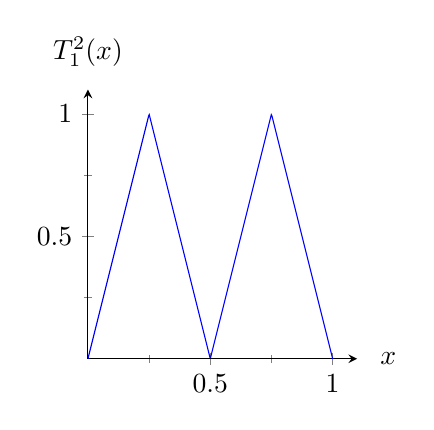
\begin{tikzpicture}
\begin{axis}[
width=5cm,height=5cm,
minor tick num=1,
axis y line=middle,
axis x line=middle,
xlabel=$x$,ylabel=$T^2_1(x)$,
every axis x label/.style={
    at={(ticklabel* cs:1.05)},
    anchor=west,
},
every axis y label/.style={
    at={(ticklabel* cs:1.05)},
    anchor=south,
},
xmin=0,
xmax=1.1,
ymin=0,
ymax=1.1
]
	\addplot[blue,mark=none,
		 domain=-0:1,samples=400] 
		{1-max(2*(1-max(2*x-1, 1-2*x))-1, 1-2*(1-max(2*x-1, 1-2*x)))};
\end{axis}
\end{tikzpicture}

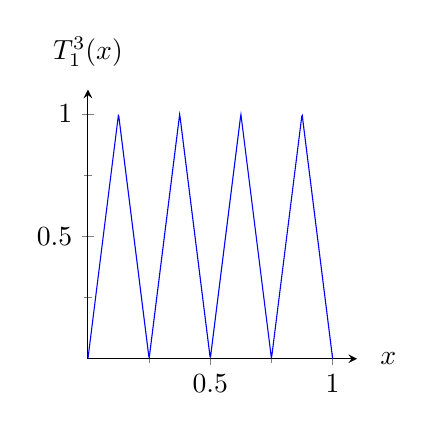
\begin{tikzpicture}
\begin{axis}[
width=5cm,height=5cm,
minor tick num=1,
axis y line=middle,
axis x line=middle,
xlabel=$x$,ylabel=$T^3_1(x)$,
every axis x label/.style={
    at={(ticklabel* cs:1.05)},
    anchor=west,
},
every axis y label/.style={
    at={(ticklabel* cs:1.05)},
    anchor=south,
},
xmin=0,
xmax=1.1,
ymin=0,
ymax=1.1
]
	\addplot[blue,mark=none,
		 domain=-0:1,samples=500] 
		{1-max(2*(1-max(2*(1-max(2*x-1, 1-2*x))-1, 1-2*(1-max(2*x-1, 1-2*x))))-1, 1-2*(1-max(2*(1-max(2*x-1, 1-2*x))-1, 1-2*(1-max(2*x-1, 1-2*x)))))};
\end{axis}
\end{tikzpicture}
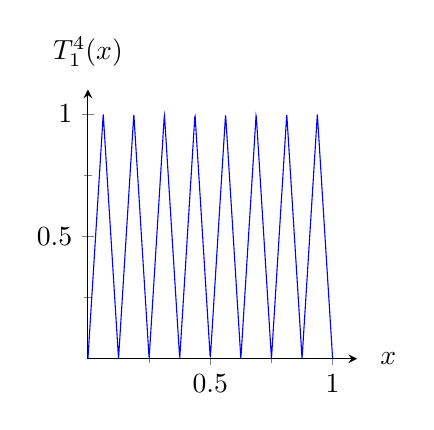
\begin{tikzpicture}
\begin{axis}[
width=5cm,height=5cm,
minor tick num=1,
axis y line=middle,
axis x line=middle,
xlabel=$x$,ylabel=$T^4_1(x)$,
every axis x label/.style={
    at={(ticklabel* cs:1.05)},
    anchor=west,
},
every axis y label/.style={
    at={(ticklabel* cs:1.05)},
    anchor=south,
},
xmin=0,
xmax=1.1,
ymin=0,
ymax=1.1
]
	\addplot[blue,mark=none,
		 domain=-0:1,samples=800] 
		{1-max(2*(1-max(2*(1-max(2*(1-max(2*x-1, 1-2*x))-1, 1-2*(1-max(2*x-1, 1-2*x))))-1, 1-2*(1-max(2*(1-max(2*x-1, 1-2*x))-1, 1-2*(1-max(2*x-1, 1-2*x))))))-1, 1-2*(1-max(2*(1-max(2*(1-max(2*x-1, 1-2*x))-1, 1-2*(1-max(2*x-1, 1-2*x))))-1, 1-2*(1-max(2*(1-max(2*x-1, 1-2*x))-1, 1-2*(1-max(2*x-1, 1-2*x)))))))};
\end{axis}
\end{tikzpicture}
\end{document}